\chapter{Einführung}

\section{Bildgebende Verfahren}
\begin{quote}
	''Die Medizinische Bildverarbeitung hat das Ziel, medizinische Bilder und Bildfolgen zur Unterstützung der medizinischen Diagnostik und Therapie aufzubereiten, zu analysieren und zu visualisieren.'' - \cite{MedBildVerarbeitung}
\end{quote}
Die verschiedenen Verfahren können in die Art der erzeugten Bilddaten eingeteilt werden:
\begin{itemize}
	\item \textbf{Schnittbilder} z.B. mittels Computertomografie, Magnetresonanztomografie oder Röntgentomografie.
	\item \textbf{Projektionsbilder} z.B. durch ''klassisches'' Röntgen.
	\item \textbf{Oberflächenabbildungen} z.B. durch Rastertunnelmikroskop.
\end{itemize}
Da das Hauptaugenmerk dieser Arbeit liegt auf der aus den tomographischen Verfahren erhaltenden Schnittbildern welche als sogenannte Voxel-Daten gespeichert werden. Ein vollständiges dreidimensionales Bild besteht aus mehreren solcher übereinandergelegten Schnittbildern.

\section{Volumengrafik}
Unter Volumengrafik versteht man in der Computergrafik die Darstellung von Objekten durch eine Menge von Voxeln. 
\\\\
Ein solches Voxel ist als ein einzelner Punkt in einem dreidimensionalen Objekt zu verstehen, welcher einen gewissen Dichtewert aufweist. Dieser Wert ist essentiell um z.B. bei den tomographischen Verfahren in der Medizin die festeren von den weicheren teilen des Körpers zu unterscheiden (z.B. Knochen und Gewebe). In Abbildung \ref{fig:Voxelgitter} ist eine solche Voxel-Menge zusehen die verschiedenen Grauwerte der einzelnen Bildpunkte stellen dabei die werte der Dichte dar.

\begin{figure}
	\centering
	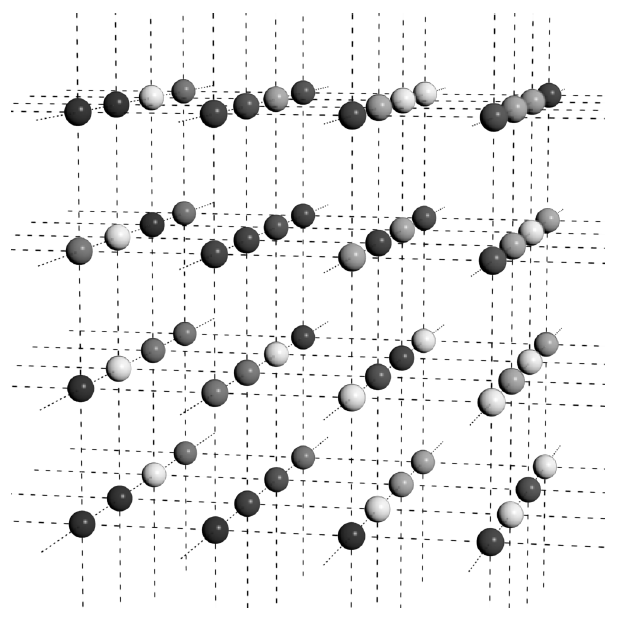
\includegraphics[width=.85\textwidth]{Voxelgitter}
	\caption{Ein Voxelgitter \cite{SeibtBak}.}
	\label{fig:Voxelgitter}
\end{figure}

\section{Marching Cubes}
Der Marching Cubes Algorithmus wurde erstmals 1988 vorgestellt (\cite{MCAlgo}). Ziel dieses Algorithmus ist die Extraktion von Isoflächen aus Volumendaten. Formal ist die Extraktion wie folgt definiert: 
\\\\
Aus einer Funktion $\varphi : \mathbb{R}^{n} \rightarrow \mathbb{R }$ wird, gegeben ein Schwellwert   c $\epsilon$ $ \mathbb{ R} $, eine
Isofläche $S_{c}$ extrahiert, für die gilt:
\begin{equation}
S_{c} := \{ \vartheta \text{ } \epsilon \text{ } \mathbb{R}^{n} \text{ | } \varphi(\vartheta) = c\}
\end{equation} 
(vgl. \cite{SeibtBak})

\subsection{Funktionsweise}

\section{Dateiformate}
Die zu dieser Arbeit herangezogenen Dateiformate sind einerseits die von dem Softwarepaket Analyze\footnote{https://rportal.mayo.edu/bir/} verwendeten Image und Header Files sowie die sogenannte STereoLithography-Schnittstelle. 

\subsection{Image File (.img)}
Diese Datei ist vergleichsweise einfach aufgebaut und enthält ein Objekt bestehend aus (normalerweise) unkomprimierten Pixel Daten (vgl. \cite{AnalyzeFormat}). Jedes Pixel repräsentiert eine Voxel mit dem dazugehörigen Dichtewert. Das Gesamte Objekt kann somit in eine 3x3 Matrix eingelesen und verarbeitet werde.

\subsection{Header File (.hdr)}
Diese Datei beschreibt die Ausmaße der Pixel-Datei sowie ihre Historie. (vgl. \cite{AnalyzeFormat}). \\\\
Die genaue Struktur nach \cite{AnalyzeFormat} ist in drei Teilbereiche aufgeteilt. Der erste Teil ist der sogenannte 

\subsection{STereoLithography (.stl)}
\begin{quote}
	''The STL (STereoLithography) file format, as developed by 3D Systems, has been widely used by most Rapid Prototyping (RP) systems and is supported by all major computer-aided design (CAD) systems.'' - \cite{STereoLithography}
\end{quote}
Eine STL-Datei besteht aus einer liste von Dreiecken. Jedes Dreieck wird durch seine drei Eckpunkte im Raum sowie durch seinen Normalvektor beschrieben. Dies führt folglich zu einer Summe von 12 Werten pro Dreieck.\\
\\
Zum besseren Verständnis kann in Abbildung \ref{fig:ASCIISTL} der Aufbau einer solchen Datei als ASCII Darstellung betrachtet werden. Für ein besseres Verständnis hinsichtlich der Implementierung ist in Abbildung \ref{fig:BINARYSTL} der Binäre Aufbau des STL-Formates zu finden. 

\begin{figure}
	\centering
	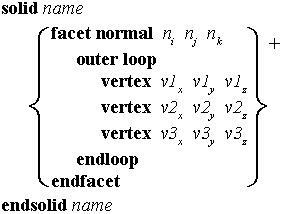
\includegraphics[width=.65\textwidth]{StL-ASCII}
	\caption{ASCII Darstellung des STL-Format \cite{STLFormat}.}
	\label{fig:ASCIISTL}
\end{figure}

\begin{figure}
	\centering
	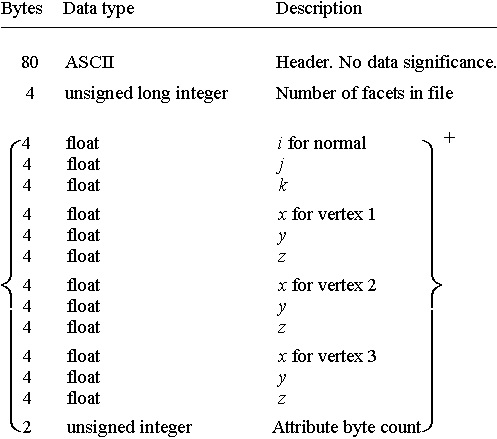
\includegraphics[width=.65\textwidth]{StL-binary}
	\caption{Binäre Darstellung des STL-Format \cite{STLFormat}.}
	\label{fig:BINARYSTL}
\end{figure}

\section{Computergrafik}
Computergrafik beschreibt das computergestützte Erstellen und Verarbeiten von Grafiken (vgl. \cite{ComputerGraphics}). 
\subsection{OpenGL}
\begin{quote}
	''OpenGL (for “Open Graphics Library”) is a software interface to graphics hardware.
	The interface consists of a set of several hundred procedures and functions
	that allow a programmer to specify the objects and operations involved in producing
	high-quality graphical images, specifically color images of three-dimensional
	objects.'' - \cite{OpenGLDoku}
\end{quote}
\subsection{QT (Bibliothek)}